\documentclass[a4paper, 12pt]{article}
\usepackage[english, slovak]{babel}
%\usepackage[T1]{fontenc}
\usepackage[utf8]{inputenc}
\usepackage[margin=1.5cm]{geometry}
\usepackage{amsmath}
\usepackage{amssymb}
\usepackage{mathrsfs}
\usepackage{listings}
\usepackage{hyperref}
\usepackage{textcomp}
\usepackage{wrapfig}
\usepackage{graphicx}
\usepackage{subcaption}
\usepackage{float}

\def\header{ % hlavička stránky
\begin{center}
Mário Lipovský \hfill Machine Learning 2017\\
\today\hfill \textbf{Semestral project}
\end{center} \vspace{-4pt}\hrule
}

\newcommand{\rowstyle}[1]{\gdef\currentrowstyle{#1}%
  #1\ignorespaces
}

\title{Classification of Calendar Events \\ 
\normalsize{Machine Learning Course Project}}
\date{January 2018}
\author{Mário Lipovský}

\begin{document}
\selectlanguage{english}
\maketitle

\begin{abstract}
The initial goal of this project was to explore a collection of events 
recorded in my personal Google calendar and to categorize them. 

% As it turned out, we devoted most of our time to preparing the dataset
% and then to simple classification tasks.
Based on keywords in the event descriptions we semi-manually labeled a 
subset of events and then used SVMs and random forests (and marginally 
tree boosting and multilayer perceptrons) to solve a classification task:
prediction of the event category based on its start time, duration.
In the final stage of the project we also created PCA-based word vectors 
of short event descriptions and achieved 80\% classification accuracy.

% This project mainly documents the pitfalls and tribulations of a student 
% who is starting with machine learning.
\end{abstract}

\section{Introduction}
In the period between November 2014 and March 2017 I have been recording most of
my daily activities (sleep, learning, leisure activities, ...) in a Google calendar
which resulted in approximately 6000 calendar events. As my project I chose to 
analyze this data.

My initial idea was to discover some behavioral patterns and try to predict the
next action I would do based on historic data. However to be able to do this,
I would need some categorization of the activities
% and the best solution for prediction would probably be a recurrent network 
% which was not covered by the course. 
So I postponed the event prediction, and focused mainly on
event categorization and classification. Thus the main goals of this project
were to prepare and explore the dataset and to try to categorize events. 

I ended up with a semi-manual categorization (I categorized events based
on manually selected keywords in summaries), but as a machine learning 
exercise I also trained multiple classifiers to validate the categorization
(to check whether ML models can distinguish these categories) and used these
classifiers to categorize uncategorized events.

\medskip

In this project we first prepare the dataset of 6075 events -- we process calendar 
\texttt{.ics} files and for each event we extract its start timestamp, 
duration and a short summary text.

To gain a bit of insight we visualize the dataset and train simple 
classification models which use numeric attributes (date, time, duration)
to map each event to one of three categories -- sleep, school, personal.
During the data collection period we separated events into three calendars
so these labels are based on calendar names. We achieve 70\% accuracy.

Based on event summaries we semi-manually label a subset of 4243 events into 
six categories and then we train classifiers from numeric attributes 
into these six categories. Here we achieve only 50\% accuracy, since 
multiple categories were indistinguishable only with use of numeric attributes.

Finally we construct word vectors from summary texts with use of PCA on bag of words. 
We use these vectors as additional event attributes in six-category
classification task. With use of word vectors we achieved 78\% accuracy
and we eventually used these models in an attempt to categorize uncategorized events.

\medskip
As the calendar information are personal, we do not include them in the repository.

\section{Dataset Preparation}
Our first task was to convert three calendar files 
\texttt{sleep.ics}, \texttt{school.ics} and \texttt{personal.ics} into a usable
dataset in form of table of all events. From each event we extracted its start
timestamp, end timestamp and a short summary text and preprocessed them.

\subsection{Attribute Preprocessing}
We decided to use the following attributes to represent a start timestamp:
\begin{itemize}
\setlength\itemsep{0.1em}
\item \texttt{minutes\_of\_day} (integer in range $0 - 24 \times 60$). 
Since people live in a daily cycle, the time of the day is very 
important attribute as it enables to associate events that occur 
in the same part of the day.
\item \texttt{weekday} (integer in range 0 -- 6, 0 is Sunday). The weekly cycle and most 
importantly weekends influence the human behaviour and so should be considered.
\item \texttt{day\_number} -- number of days since Jan 1st 2014. We added this
attribute so that events which happened in a similar time period would have
something similar and also so that events which happened on different days
would be distinguishable. Thanks to this attribute it might be possible to observe
long term trends.
\end{itemize}

Instead of using start and end timestamps, we use start time and duration.
An event may start and end on different days (e.g. sleep) and as we use multiple
attributes to represent a timestamp, it might be almost impossible for
a model to reconstruct duration from start and end attributes. 

We represent duration with one integer in minutes \texttt{duration\_minutes}.

\medskip

As the summaries are mostly in Slovak language, we first removed diacritics.
Since the upper case is used inconsistently (as the first character of summary
or as a person's name), we lower-cased the summaries. Finally we replaced all
characters except \texttt{a-z0-9\_} with a space and we removed repeated, leading
and trailing spaces. Although we decided to keep the numbers to allow detection
of some university room names (e.g. t2, f1), we later discarded most of
them (at removal of short words in word vector preprocessing).

\medskip 

For each event we also included a name of the source calendar file (sleep, school
or personal) that can be used as a simple classification label.

\medskip

Applying this procedure we produced a single file with 6075 events
where each event is characterized by 
\texttt{summary}, \texttt{day\_number}, \texttt{weekday}, \texttt{minutes\_of\_day},
\texttt{duration\_minutes} and \texttt{label}. There are 10 randomly selected data 
points shown in the following table:

\begin{footnotesize}
\begin{verbatim}
                          summary  day_number  weekday  minutes_of_day  duration_minutes     label
                         cvicenie         714        2            1410              30.0  personal
  neurodrogy stavba mozgu neuronu         778        3            1290              90.0  personal
              citanie o meditacii         670        0             780              60.0  personal
                             riad        1084        1            1110              30.0  personal
      cesta do ba ucenie sa sieti         823        6             600             120.0    school
libetov experiment s rp a vedomim         689        5             900              90.0    school
             bakalarsky seminar 1        1050        2             690              60.0    school
           skolemov normalny tvar         724        5             690              60.0    school
                           spanok         413        2               0             480.0     sleep
                           spanok        1017        4              60             270.0     sleep
\end{verbatim}
\end{footnotesize}

\section{Three-class Classification}
At first we didn't use the summaries and we tried to solve the classification task
where the inputs $X$ consisted of numeric attributes: $X_i = ($\texttt{day\_number}, 
\texttt{weekday}, \texttt{minutes\_of\_day}, \texttt{duration\_minutes}$)$ and the 
labels $y$ were the calendar names: $y_i := $ \texttt{label}.

4172 events were from personal calendar, 985 were from school calendar, 
and 917 events from sleep calendar.
    
\subsection{Dataset Visualization}
\begin{figure}[h]
\centerline{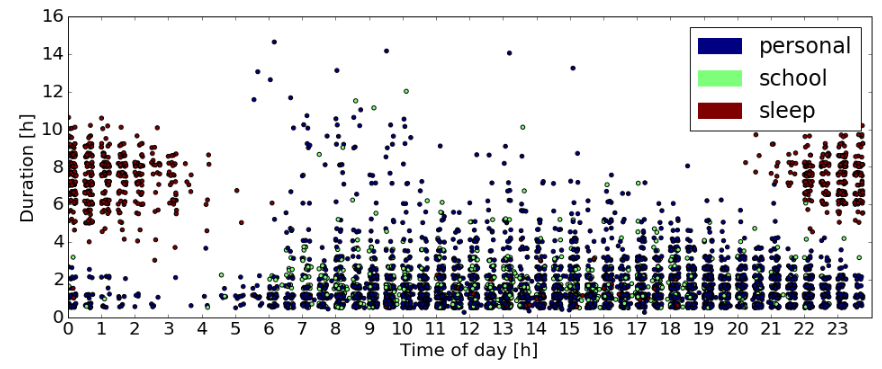
\includegraphics[width=1\textwidth]{3class-duration-vs-tod.png}}
\caption{The distribution of events of different durations and at different times
of day. As most events have their start times and durations rounded to 15 minutes
(XX:00, XX:15, XX:30, XX:45), to visualize multiple points per (t.o.d. $\times$ 
duration) we add small random noise to points.}
\end{figure}

In Figure 1 we can see that most of the sleep events are easily distinguishable because of their long
duration and night time, but a few sleep events also occur during the day after lunch.
The school and personal events don't seem to be separable, although there is 
considerably fewer school events after 19:00.

\begin{figure}[h!]
\centerline{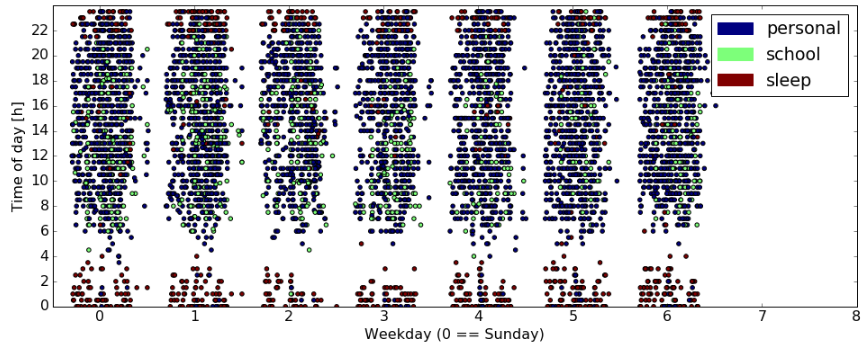
\includegraphics[width=1\textwidth]{3class-tod-vs-weekday.png}}
\caption{The distribution of events at different different times of day on different 
weekdays. Here we add randomness only in $x$ coordinate. The data in this projection 
shows similar patterns as in Fig.1.}
\end{figure}

Although we might expect fewer school events during the weekends in Figure 2,
we did not include the lecture (repeated) events and so all school events correspond to
homeworks and learning which is spread throughout the whole week.
The students can never truly rest.

The same patterns were also observable via 2D PCA -- distinguishable sleep,
indistinguishable school and personal and area without much school.

\subsection{Classification}
We tried to train a Support Vector Machine (SVM) with gaussian kernel and 
a Random Forest Classifier (RFC). 

\medskip

To indicate overfitting we split the data into training and testing in 80:20
ratio. To minimize the effect of variance we have also used 5-fold 
cross validation and we observed the mean and standard deviation of accuracies
of 5 trained instances per one setting of parameters.

We have manually tuned the parameters to achieve the highest testing accuracy.
we also tried to achieve the smallest gap between training and testing
data as it is an indicator of low variance and thus minimal overfitting.

For SVMs we changed two parameters: $C$ -- the penalty for crossing the
margin and $\gamma$ -- inverse of the width of gaussian. We fought the
overfitting by decreasing $\gamma$ and thus increasing SVM's 
generalization ability. Modifying $C$ usually only led to overfitting (larger
gap between training and testing accuracy) or to underfitting (drastic drop
in both accuracies).

For RFCs we changed $n$ -- the number of trees and $d$ -- max. depth of a tree.
Since we only used 4-dimensional examples $X_i$, for any $d<4$ the RFC underfitted
and so we only minimized the number of trees to avoid overfitting and to increase
the efficiency.

\medskip 

After the training we obtained the following results:
\begin{table}[h!]
\centering
\begin{tabular}{ l l l }
model & training accuracy & testing accuracy \\  \hline 
SVM ($C=1, \gamma=0.0001$) & 0.823 +/- 0.003  & 0.815 +/- 0.013 \\
RFC ($n=20, d=4$) & 0.813 +/- 0.003 & 0.813 +/- 0.013    
\end{tabular}
\end{table}


\begin{figure}[h!]
\centering
\begin{subfigure}{.5\textwidth}
  \centering
  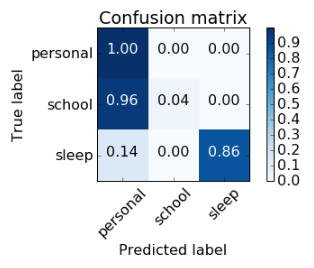
\includegraphics[width=0.8\linewidth]{3class-cm-svm.png}
  \caption{A confusion matrix for SVM.}
\end{subfigure}%
\begin{subfigure}{.5\textwidth}
  \centering
  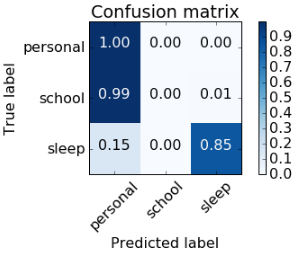
\includegraphics[width=0.8\linewidth]{3class-cm-rfc.png}
  \caption{A confusion matrix for RFC.}
\end{subfigure}
\end{figure}

A look at the confusion matrix revealed that we have a problem with
imbalanced classes (as there are 4 times more personal events than sleep or school
events) and so the accuracy is not the only metric we would want to optimize.

As the sleep events are easily separable, both models are able to successfully
categorize sleep events but fail to separate school and personal events.

\subsection{Dealing With Imbalanced Classes}
We started to use macro-F1 score as metric which would consider classes 
as equally important. F1 score allows to compare classification methods
in both specificity (precision, true positives / classified positives) and 
selectivity (recall, true positives / all positives). For macro-F1, F1 score
is first computed for each class and then the average of scores is taken, thus
assigning the same importance to each class. 

The first thing which we tried was to use boosting as it should train some
classifiers on wrongly classified examples. As the base classifier we used
RFC from the previous section. We minimized the number of RFC instances
to 10 (higer number led to overfitting, lower had small effect) but we
only achieved a slight change in confusion matrix (12\% of school events
were now successfully categorized).

As our final solution we decided to subsample training data so it would contain
approximately 1000 events from each class (we have randomly sampled $1/4$ of 
the personal events, shrinking the dataset from 6000 total examples to 3000) 
and we summarize the achieved results in the following table and confusion matrices.

\begin{table}[h!]
\centering
\begin{tabular}{ l l l l l }
model & training acc. & testing acc. & training mac-F1 & testing mac-F1 \\ \hline  
SVM ($C=1, \gamma=0.0001$) & 0.823 +/- 0.003  & 0.815 +/- 0.013 & 0.632 +/- 0.006 & 0.610 +/- 0.008\\
RFC ($n=20, d=4$) & 0.813 +/- 0.003 & 0.813 +/- 0.013 & 0.595 +/- 0.004 & 0.594 +/- 0.007\\
Boosted 10$\times$ RFC & 0.833 +/- 0.002 & 0.822 +/- 0.012 & 0.685 +/- 0.006 & 0.659 +/- 0.015\\
Subsampled SVM & 0.713 +/- 0.004 & 0.696 +/- 0.025 & 0.726 +/- 0.003 & 0.710 +/- 0.021 \\
Subsampled RFC & 0.723 +/- 0.008 & 0.699 +/- 0.021 & 0.731 +/- 0.007 & 0.707 +/- 0.018
\end{tabular}
\end{table}

\begin{figure}[h!]
\centering
\begin{subfigure}{.3\textwidth}
  \centering
  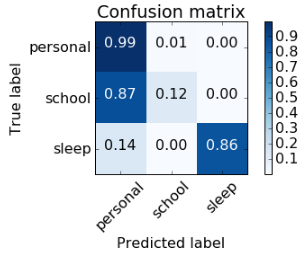
\includegraphics[width=1\linewidth]{3class-cm-boost.png}
  \caption{Boosted RFC.}
\end{subfigure}%
\begin{subfigure}{.3\textwidth}
  \centering
  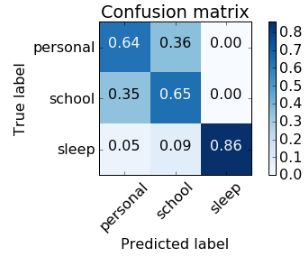
\includegraphics[width=1\linewidth]{3class-ss-cm-svm.png}
  \caption{Subsampled SVM.}
\end{subfigure}%
\begin{subfigure}{.3\textwidth}
  \centering
  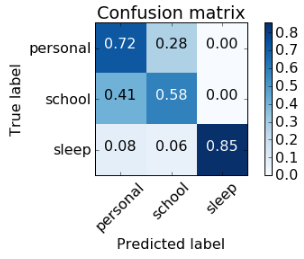
\includegraphics[width=1\linewidth]{3class-ss-cm-rfc.png}
  \caption{Subsampled RFC.}
\end{subfigure}
\end{figure}

Although with the subsampling the deviation of scores increased 
and the accuracies dropped to 70\%, the macro-F1 scores increased
and we can see from the confusion matrix that these models are much
better in distinguishing school and personal events (approximately 65\%
2-class accuracy).

Accuracies and scores were evaluated using the subsampled dataset,
but even when we trained the models on subsampled dataset and evaluated
them on the whole dataset, the confusion matrix remained almost identical
and the accuracies dropped to 66\% (effect of more personal data).

One remark for the end of section: sleep events can be discriminated with 96\%
accuracy if we treat school and personal events as one category.

\section{Six-class Classification}
The personal calendar holds events of many different types. To come closer 
to our goal, we would like to identify some more fine-grained categories 
of events in the personal calendar.

This should be possible to do with use of summary texts. Although clustering
of data-points could be done with unsupervised methods such as k-means,
we first opted for a simpler solution: semi-manual categorization based on keywords. 

\subsection{Semi-manual Categorization}
To categorize events we have printed out 200 of the most frequent words
and manually created categories (trojsten\footnote{A volunteer activity: organizing
programming competitions and camps for high-school students. Check www.trojsten.org.}, 
chores, school\footnote{A closer look on data revealed that also some school events 
were recorded in the personal calendar (in the period when the school calendar did not exist yet).
This might have caused some difficulties in the 3-class classification, although
only 300 out of 4000 personal events were categorized as school.}, work, 
active\_relax, workout, passive\_relax, food, with\_people) 
and a list of keywords for each category, e.g. \texttt{
{'}food{'}: [{'}obed{'}, {'}vecera{'}, {'}ranajky{'}, {'}pizza{'}]}.

\begin{wrapfigure}{r}{8cm}
\centering
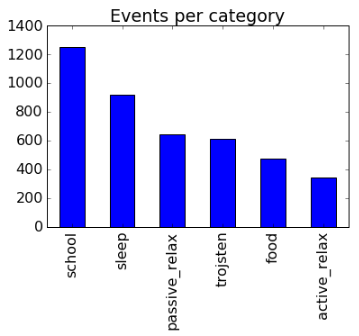
\includegraphics[width=0.9\linewidth]{events_per_category.png}
\end{wrapfigure}

Afterwards we created a list of categories for each summary -- if a summary contained
a keyword belonging to a category, this category was added to the list. Some summaries
were associated with multiple categories and this problem had to be resolved. 

It turned out that many of the summaries contained a comma separated list of 
activities, since each activity was too short to deserve its own event. 
The best solution would probably be to split each of these compound events into more 
shorter events. We, however, opted for a simpler solution -- discarding the 
events that have been assigned to multiple categories.


To minimize the losses caused by multiple-category-conflicts we reduced
the number of different categories. We discarded categories chores and work
since they contained less than 100 events. Furthermore we discarded categories
workout and with\_people since they had a lot of conflicts with food events 
(morning workout + breakfast, lunch with a person). This process has left us
with five categories: trojsten, school, food, active\_relax, passive\_relax.

When we also added the data from school and sleep calendars, we got a set
of 4243 categorized events with the distribution shown in the barplot.

\subsection{Dataset Visualization}

\begin{figure}[H]
\centerline{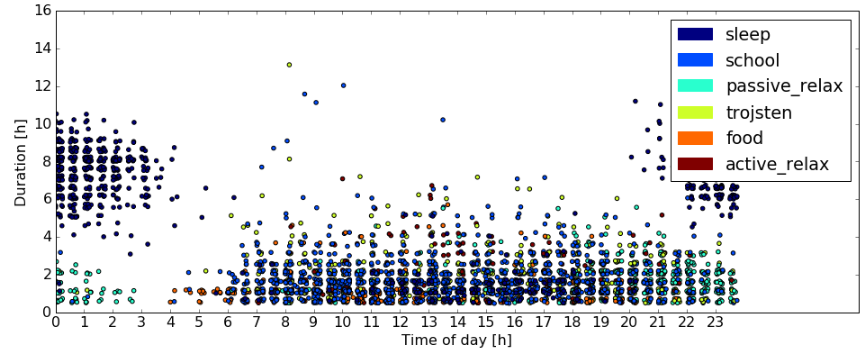
\includegraphics[width=1.1\textwidth]{6class-duration-vs-tod.png}}
\caption{The distribution of events of different durations and at different times
of day with small random noise.}
\end{figure}

With use of Figure 5 we can do some new observations.
Almost all non-sleep events that start after midnight fall into passive\_relax
category (watching a movie, reading a book, ...). The periods of time from 20:00
are filled with passive\_relax, but also some school and trojsten activities occur.
The longer events are mostly categorized as school and trojsten. Food events
are usually short and occur mostly in ranges 4:00 - 7:00, 10:00 - 15:00 and 
18:00 - 20:00. No shocking news, but it is nice what can be seen from such 
a simple plot.

\subsection{Classification}
We used the same methods for classification here as in case of three classes.
The only changes in parameters that led to better models were $\gamma = 0.00005$
(half of the previous value = wider gaussians) for SVMs and we only 
used 5 copies of RFC at boosting.

The problem of imbalanced classes again came into play so the SVM and RFC
trained on all data were unable to distinguish trojsten, food and active\_relax
(the least frequented categories) from the most frequented one -- school.
The RFC scored significantly worse here than SVM, most probably because the SVM
can formulate more sophisticated hypotheses (decision trees only cut the space
with hyperplanes that are perpendicular to the main axes).

Boosted RFC reached the same accuracy and scores as SVM -- here was boosting
used on the purpose for which it was designed, to decrease bias. The fact
that boosted RFC and SVM reached the same results (accuracy of 58\%, F1 score of 0.45) 
can hint us that this is probably the best result which we can get with all data.

To decrease bias towards frequent categories, we again subsampled data, so approximately
400 datapoints are present in each category (2400 out of total 4243 events).
The best trained model was SVM with testing accuracy of 50\% and F1 score 0.49.
The change in F1 score wasn't so high as in 3-class case (now only 0.05 points 
instead of 0.1), but as the macro F1 score is the average of F1 scores for each
class and here we have two times more classes, the change is quite comparable.
Still, the accuracies of trojsten and active\_relax classification are insufficient.

From these observations we can conclude that it is very hard to distinguish
active\_relax and trojsten activities from school and food only by using the
time and duration of events.


\begin{table}[h!]
\centering
\begin{tabular}{ l l l l l }
model & training acc. & testing acc. & training mac-F1 & testing mac-F1 \\  \hline 
SVM ($C=1, \gamma=0.00005$) & 0.606 +/- 0.003 & 0.580 +/- 0.011 & 0.482 +/- 0.004 & 0.447 +/- 0.009 \\
RFC ($n=20, d=4$) & 0.547 +/- 0.002 & 0.541 +/- 0.014 & 0.354 +/- 0.011 & 0.347 +/- 0.017 \\
Boosted 5$\times$ RFC & 0.613 +/- 0.005 & 0.583 +/- 0.014 & 0.500 +/- 0.006 & 0.451 +/- 0.014 \\
Subsampled SVM & 0.579 +/- 0.002 & 0.508 +/- 0.017 & 0.566 +/- 0.003 & 0.491 +/- 0.018 \\
Subsampled RFC & 0.509 +/- 0.002 & 0.503 +/- 0.012 & 0.441 +/- 0.012 & 0.434 +/- 0.014
\end{tabular}
\end{table}

\begin{figure}[H]
\centering
\begin{subfigure}{.5\textwidth}
  \centering
  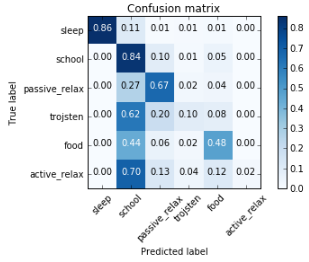
\includegraphics[width=1\linewidth]{cm1.png}
  \caption{SVM.}
\end{subfigure}%
\begin{subfigure}{.5\textwidth}
  \centering
  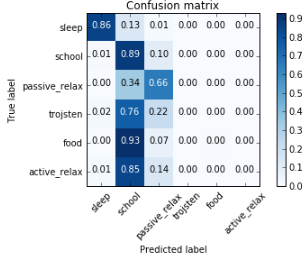
\includegraphics[width=1\linewidth]{cm2.png}
  \caption{RFC.}
\end{subfigure}
\begin{subfigure}{.5\textwidth}
  \centering
  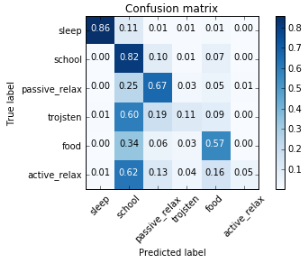
\includegraphics[width=1\linewidth]{cm3.png}
  \caption{Boosted RFC.}
\end{subfigure}
\begin{subfigure}{.5\textwidth}
  \centering
  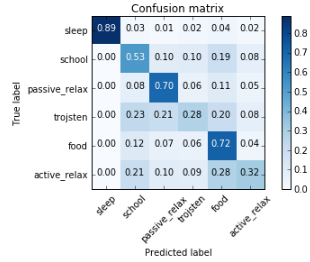
\includegraphics[width=1\linewidth]{cm4.png}
  \caption{Subsampled SVM.}
\end{subfigure}%
\begin{subfigure}{.5\textwidth}
  \centering
  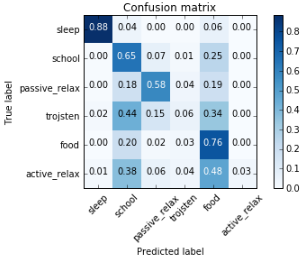
\includegraphics[width=1\linewidth]{cm5.png}
  \caption{Subsampled RFC.}
\end{subfigure}
\end{figure}


\section{Word vectors}
In this section we finally use methods of machine learning on the summaries.

We were incrementally improving the word vectors and we tried to evaluate
their quality in each stage with PCA. When the vectors were computed, we 
looked at the explained variance ration in the first 2 and 100 components,
we printed out the 5 most important words (words which had the highest
absolute value in the principal component) in the 5 most important components
and we also plotted the PCA projection to 2D.

\subsection{Gradual Improvement of Word Vectors}
We started with creating a bag of words with use of all 4701 distinct words.
Although the conjunctions and prepositions were considered as most important words,
the first 100 components already captured 47\% of all variance (of all information).
In the 2D projection most of sleep events and also a lot of trojsten
events are easily separable and other events create some clusters.

\begin{small}
\begin{verbatim}
Explained variance ratio in    2 components 0.079192669504
Explained variance ration in 100 components 0.471266889902
5 most important words in first 5 components:
['spanok', 'a', 's', 'obed', 'o']
['a', 's', 'spanok', 'obed', 'vecera']
['s', 'ksp', 'a', 'obed', 'o']
['s', 'a', 'o', 'ranajky', 'cvicenie']
['o', 'ranajky', 'cvicenie', 'sprcha', 'ksp']
\end{verbatim}
\end{small}

\medskip

In the second step we tried to remove stop words -- unimportant words, usually those
that often repeat in text. When we removed all short words (with lengths 1, 2)
and all words with less than three occurrences, we were left with 855 words and now
the first 100 components captured almost 60\% of variance. In 2D projection
clear clusters of food events and passive\_relax events were formed.

\begin{small}
\begin{verbatim}
Explained variance ratio in   2 components 0.116129541457
Explained variance ratio in 100 components 0.597728010393
5 most important words in first 5 components:
['spanok', 'ksp', 'obed', 'gitara', '9gag']
['ranajky', 'sprcha', 'cvicenie', 'ksp', 'proofread']
['ksp', 'ranajky', 'cvicenie', 'sprcha', 'obed']
['gitara', 'obed', '9gag', 'ksp', 'film']
['gitara', 'film', 'obed', 'the', 'ksp']
\end{verbatim}
\end{small}

\medskip

Finally we used a Slovak stemmer from \texttt{https://github.com/mrshu/stemm-sk}
to first stem all words, and then we removed all short and infrequent words.
This approach led to 80\% of explained variance in the first 100 components.

\begin{small}
\begin{verbatim}
Explained variance ratio in   2 components 0.234588594894
Explained variance ratio in 100 components 0.808329433367
5 most important words in first 5 components:
['spanok', 'ksp', 'obed', '9gag', 'film']
['ksp', 'proofread', 'obed', '9gag', 'film']
['obed', '9gag', 'film', 'ksp', 'the']
['9gag', 'obed', 'film', 'the', 'ksp']
['film', '9gag', 'the', 'ksp', 'obed']
\end{verbatim}
\end{small}

\subsection{Classification}
Eventually we trained SVM, RFC and Multilayer Perceptron (with ReLu units,
100 and 50 neurons on hidden layers and optimized with Adam) on word vectors (v)
and then on word wectors combined with numeric data (v + n) and finally
on subsampled data (v + n sumsampled). All methods achieved approximately 80\% accuracy and F1 score
in range of 0.75 to 0.8.

\begin{table}[h!]
\centering
\begin{tabular}{ l l l l l }
model & training acc. & testing acc. & training mac-F1 & testing mac-F1 \\  \hline \hline 
v SVM & 0.818 +/- 0.002 & 0.808 +/- 0.010 & 0.760 +/- 0.001 & 0.748 +/- 0.009 \\  
v RFC & 0.815 +/- 0.003 & 0.804 +/- 0.007 & 0.755 +/- 0.003 & 0.743 +/- 0.010 \\ 
v MLP & 0.823 +/- 0.002 & 0.811 +/- 0.009 & 0.767 +/- 0.001 & 0.752 +/- 0.008  \\ \hline 
v + n SVM & 0.860 +/- 0.002 & 0.802 +/- 0.012 & 0.818 +/- 0.003 & 0.756 +/- 0.010 \\                 
v + n RFC & 0.833 +/- 0.002 & 0.818 +/- 0.013 & 0.781 +/- 0.005 & 0.761 +/- 0.014 \\                 
v + n MLP & 0.868 +/- 0.004 & 0.825 +/- 0.022 & 0.856 +/- 0.004 & 0.811 +/- 0.019 \\ \hline 
v + n subsampled SVM & 0.810 +/- 0.004 & 0.743 +/- 0.022 & 0.820 +/- 0.003 & 0.758 +/- 0.019 \\                 
v + n subsampled RFC & 0.826 +/- 0.004 & 0.784 +/- 0.017 & 0.837 +/- 0.003 & 0.797 +/- 0.016 \\
v + n subsampled MLP & 0.842 +/- 0.003 & 0.785 +/- 0.019 & 0.842 +/- 0.004 & 0.786 +/- 0.021
\end{tabular}
\end{table}

\subsection{Labeling of unlabeled data}
The classification models could be used for labeling of uncategorized data.
Here we only show a few examples. Also, because of time pressure we did not
evaluate this labeling in any way (apart from marking with \texttt{*} the labels which we 
consider as correct).

\begin{small}
\begin{verbatim}
                                      summaries categories SVM  categories RF categories MLP
                zapis stipendium diplomy na gjh         school*      trojsten          sleep
                      prve 2 kapitoly z algebry         school*        school*        school*
                                 gjh ocenovanie       trojsten       trojsten       trojsten
                      trojstenovy pondeok kvizy         school         school         school
                                  d u programko         school*        school*        school*
                                           riad           food           food   active_relax
                                 55 vyrocie gjh       trojsten       trojsten       trojsten
                                      vysavanie         school         school         school
                                       aj uloha         school*        school*        school*
                            cvicenia z matalyzy         school*        school*        school*
                                           heno         school         school         school
                                            ...            ...           ...             ...
                                     kapustnica         school         school         school
pomoc na akademii veci do skoly ak nebude treba         school*        school*        school*
                                            vub         school         school  passive_relax
                                     webstretko   active_relax         school       trojsten*
                                         aupark   active_relax*        school       trojsten
                               party byrokratov   active_relax*        school       trojsten*
                                    organizacia         school         school         school
                ml engineer s look at insurance   active_relax         school       trojsten
                      posedenie s janom a petou   active_relax*        school       trojsten*
                          matfyzacka kapustnica         school*        school*      trojsten
\end{verbatim}
\end{small}

\section{Ideas For Improvement}

\subsection{Format of Time-denoting Attributes}
Instead of coding Sunday, \dots, Saturday as 0, \dots, 6 it would have been 
probably better to code Monday as 0 and Sunday as 6, since 
Saturday and Sunday are similar days (they are both free) and so they 
should be denoted with similar values.

\medskip

It might also be helpful to add \texttt{month\_of\_year}, but since the data cover
only a period of two years, characteristics of each month are probably not observable 
or the trends can be expressed with use of \texttt{day\_number}. People usually
don't even realize which \texttt{day\_of\_year} is today and 
don't make decisions only based on \texttt{day\_of\_month} so we considered these
attributes as uninformative (although we didn't experimentally prove it).

\subsection{Unused Calendar Information}
All calendar events also contain timestamp of its creation and last modification.
For simplicity we decided to not to take these timestamps into account, 
but it might be interesting to also consider the creation 
timestamp in relationship to start time, since it might help to distinguish 
planned and unplanned events. 

Since only very few ($<20$) of the calendar events include the location
information and a longer description, these information were discarded. 

Google calendar allows creation of repeated events (e.g. lectures).
To consider such events, one record would have to be transformed into multiple
records (one calendar event per occurrence). As this would require a bit more
engineering and also it might cause our models to overfit repeated events, we decided
to not implement this feature and we did not process repeated events.
If we would include these events to the dataset we would add a binary attribute 
denoting whether an event is repeated and maybe the number of occurrences. 
Since almost all repeated events occur weekly, we would not include frequency.

The dataset could be further enhanced by other relevant information such as
the times of sunrise and sunset (which might influence the sleep) or the weather
during the day (which might influence in-door and out-door activities).


\end{document}
